%!TEX root = pag0.tex
\chapter{Algoritmo}
\label{chapter4}

Lo scopo del progetto è di tracciare e stimare la posizione 3D del pulsante desiderato durante il moto del braccio utilizzando una camera monoculare. 
Come definito nel capitolo ~\ref{chapter1} la camera non fornisce informazioni sulla profondità. Per ottenere la posizione 3D date le informazioni 2D del pulsante si utilizza un algoritmo esterno detto PTAM. 
Per gestire i due algoritmi si utilizza il framework ROS atto a far comunicare più algoritmi contemporaneamente tramite l'invio di messaggi. 
In figura ~\ref{fig:struttura} si è schematizzata la struttura dell'algoritmo.
\begin{figure}[H]
   \centering
   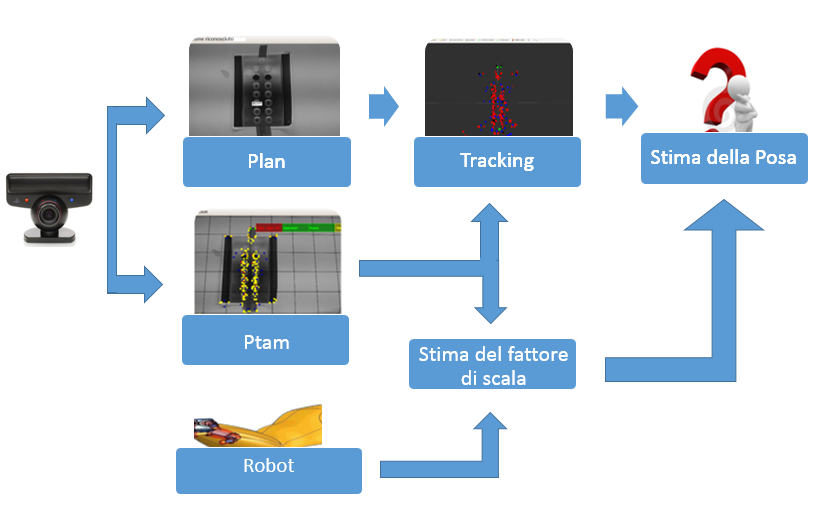
\includegraphics[width=0.9\columnwidth]{struttura.png} 
   \caption{Struttura dell'algoritmo sviluppato}
   \label{fig:struttura} 
\end{figure}
La prima parte è dedicata al riconoscimento delle forme geometriche nella scena e all'interazione con l'utente. La seconda parte è dedicata al tracking dell'oggetto desiderato nei successivi frame. L'ultima parte ricerca la posizione 3D del oggetto utilzzando sia le informazioni provenienti da PTAM, sia le informazioni sullo spostamento reale del robot. Nell'allegato ~\ref{Appendix} vengono mostrati le strutture degli algoritmi implementati.

\subsection{Fase di plan}
La telecamera invia lo streaming della scena al nodo Ros di PTAM e contemporaneamente invia un immagine statica, della stessa scena, al nodo da noi creato. Con questa immagine statica siamo in grado di riconoscere i contorni delle immagini tramite il filtro di Harris ~\cite{Harry}. Questo filtro è basato sull'approssimazione del auto-correlazione del gradiente in diverse direzioni. Per ogni contorno trovato si calcola i centri di massa e si verifica quale tra questi centri ha la minor distanza euclidea dal punto premuto dal utente. Dall'immagine si estrapola la zona dell'oggetto interessato e si calcolano le features e i relativi descrittori utilizzando il filtro Sift. Nella figura ~\ref{fig:fase_plan} si può vedere un esempio di questo algoritmo. 
\begin{figure*}
  \centering
   \subfigure[$Scena\_iniziale$]{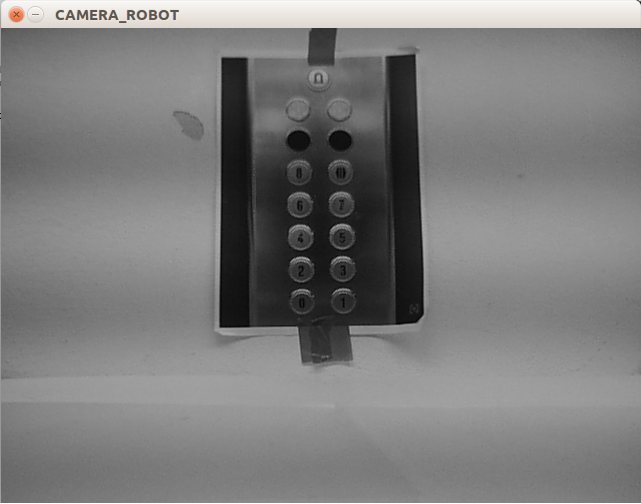
\includegraphics[width=.8\hsize]{fase1}\label{fig:scene}}
  \subfigure[$Bottone\_scelto$]{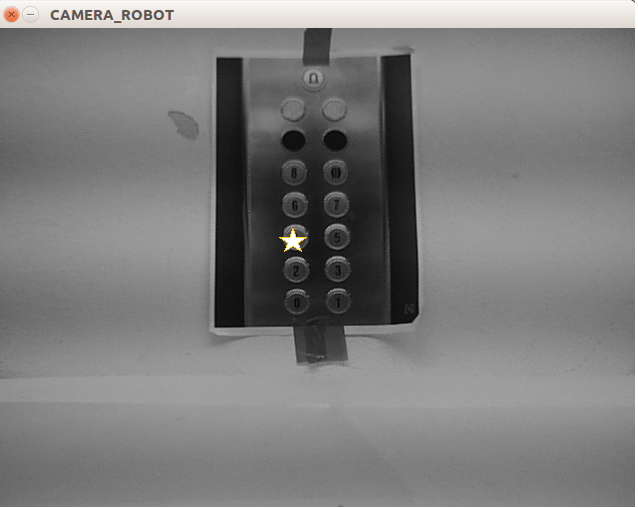
\includegraphics[width=.8\hsize]{bottonescelto}\label{fig:BottoneScelto}}
\end{figure*}
\begin{figure*}
  \centering  
  \subfigure[$Figure\_trovate$]{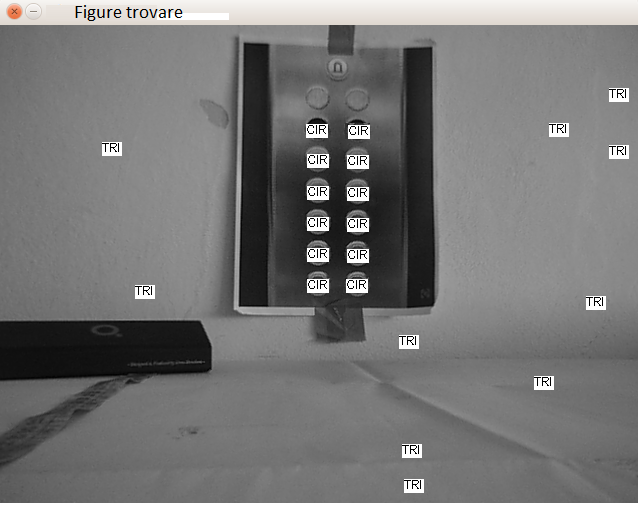
\includegraphics[width=.8\hsize]{figureTrovate}\label{fig:FigureTrovate}}
  \subfigure[$Bottone\_riconosciuto$]{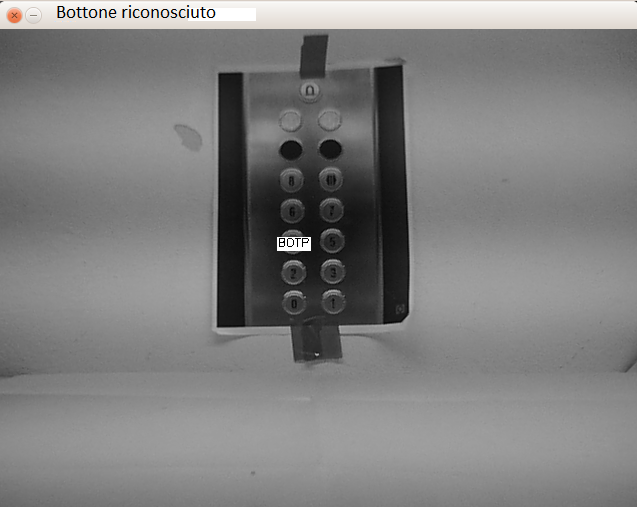
\includegraphics[width=0.8\hsize]{bottone_riconosciuto}\label{fig:bottonericonosciuto}}
  \caption{Esempio di ricerca del bottone selezionato}
  \label{fig:fase_plan}
\end{figure*}

\newpage
\subsection{Fase di tracking}
Quando il robot si muove invia un messaggio con la posa rispetto al frame precedente. In questo modo si tiene traccia dei reali spostamenti del robot. Nel nuovo frame si ricalcolano i descrittori dell'intera immagine e si calcola il match con le features del pulsante riconosciuto precedentemente. Il match è stato calcolato tramite il metodo FLANN acronimo di ~\emph{fast approximate nearest neighbor} ~\cite{FLANN}. Questo metodo consiste nel trovare i punti vicini tramite una ricerca randomica dell'albero creato. Utilizzando i migliori descrittori, che realizzano il matching, si calcola il centroide di questi punti. Questo nuovo punto rappresenta la posizione del pulsante nel nuovo frame. Ad ogni iterazione si esegue il matching con il pulsante trovato nella prima immagine.
In figura ~\ref{fig:fase_tracking} si può vedere un esempio del matching per il compito in esame. Come si può notare dalla figura ~\ref{fig:Matching} i descrittori trovati possono essere molti, anche distanti dalla zona di interesse. Per questa ragione si utilizza un controllo aggiuntivo basato sulle distanze per minimizzare questo numero. In figura ~\ref{fig:Good_matching} si mostrano i punti trovati utilizzando il controllo aggiuntivo. Questo controllo aggiuntivo fa in modo che la distanza euclidea dei punti del match non superi mai una soglia imposta. In questo modo riusciamo ad eliminare possibili outlier e a ridurre il campo di ricerca.     
\begin{figure*}
  \centering
  \subfigure[$Sift\_frame2$]{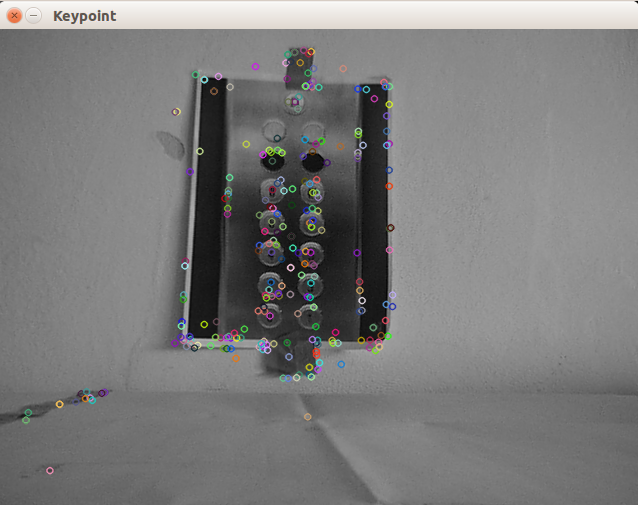
\includegraphics[width=.8\hsize]{keypoint}\label{fig:sift_scene2}}
  \subfigure[$Matching$]{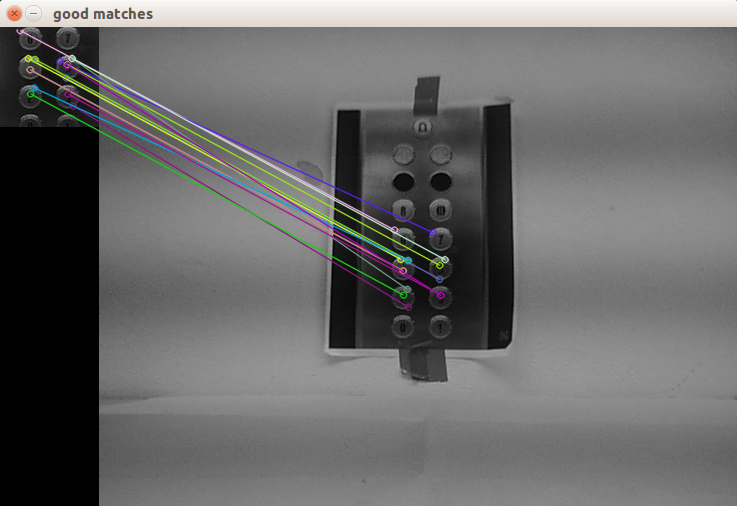
\includegraphics[width=.8\hsize]{match1}\label{fig:Matching}}
\end{figure*}
\begin{figure*}
  \centering  
  \subfigure[$Good\_matching$]{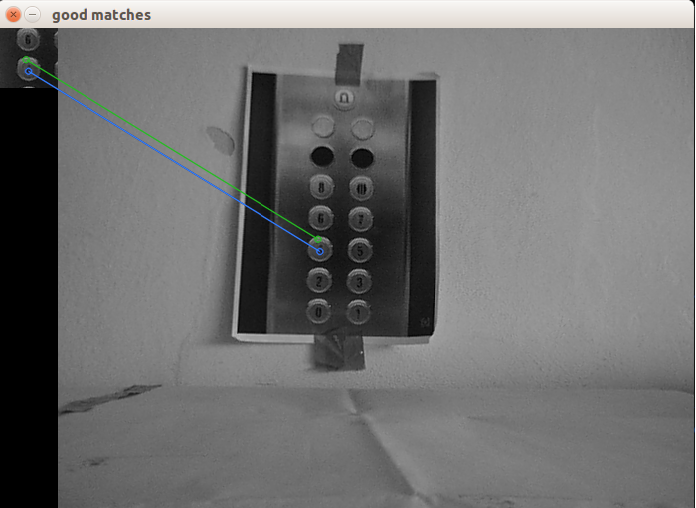
\includegraphics[width=.8\hsize]{goodmatch}\label{fig:Good_matching}}
  \subfigure[$Botton\_frame2$]{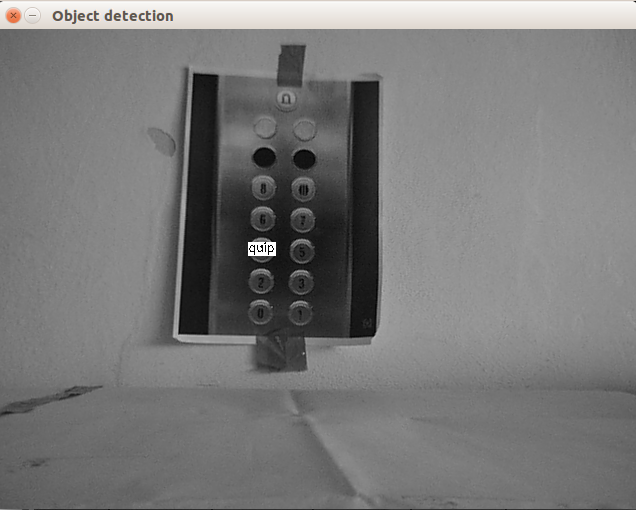
\includegraphics[width=.8\hsize]{bottone2frame}\label{fig:Botton_frame2}}
  \caption{Tracking del pulsante}
  \label{fig:fase_tracking}
\end{figure*}

\newpage
\subsection{Fase di interazione}
\subsubsection{Ptam}
Per spiegare come si è ottenuta la posa del pulsante rispetto alla telecamera, occorre spiegare come funziona l'algoritmo PTAM. Questo algoritmo è usato per la realtà aumentata e può essere riassunto da:
\begin{itemize}
\item Tracking delle features in ogni frame
\item Mapping delle features
\end{itemize}
Una mappa è un insieme di $M$ features rispetto al frame \lq \lq mondo\lq\lq $W$. Ogni features rappresenta un punto nel mondo 3D con coordinate $p_{jw} = (x_{jw} , y_{jw} , z_{jw}, 1)^t$ rispetto al frame W. La mappa è creata in fase di inizializzazione tramite la stereo visione. Come spiegato nel capitolo ~\ref{chapter2} la stereo visione è la stima della profondità tramite l'utilizzo di due immagini della stessa scena prese da angolazioni differenti. Durante la fase di inizializzazione la camera viene mossa sull'asse orizzontale, così facendo si tracciano le features durante lo spostamento e si stima la posizione 3D tramite algoritmi randomici. Un esempio di questa inizializzazione è mostrato in figura ~\ref{fig:fase_init}.
\begin{figure}[H]
   \centering
   \subfigure[$Fase\_init$]{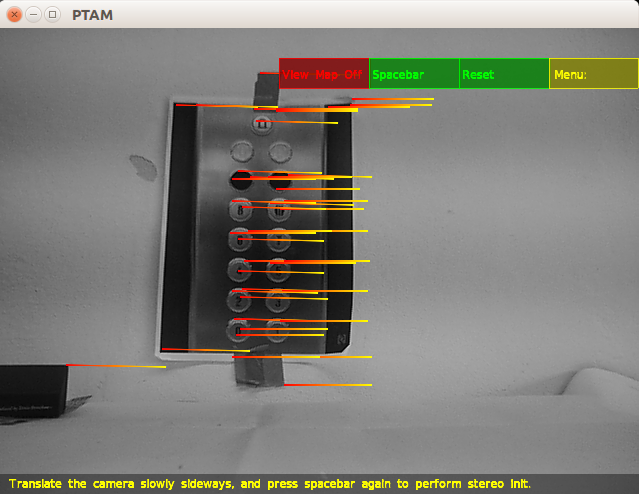
\includegraphics[width=.8\hsize]{ptaminit}\label{fig:fase_init}}
   \subfigure[$Ptam\_grid$]{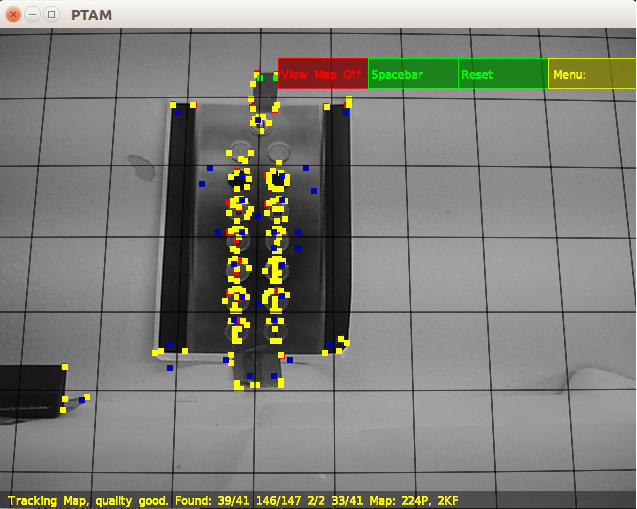
\includegraphics[width=.8\hsize]{ptamgrid}\label{fig:first_ptam_gird}}
   \caption{Fsse di inizializzazione di PTAM}
   \label{fig:fase_init} 
\end{figure}

Oltre alla posizione 3D delle features, figura ~\ref{fig:rviz_Fpoint}, rispetto al frame word questo algoritmo fornisce la posa della camera rispetto al frame W  ~\ref{fig:rviz_frame}. Questa posa è calcolata iterativamente minimizzando una funzione obbiettivo dato dall'errore di riproiezione nel piano immagine:
\begin{equation}
\mu = \argminB_\mu {\sum_{j \in S} Obj(\frac{|e_j|}{\sigma},\sigma_t)}
\label{eq:funzione obbiettivo}
\end{equation}
Dove $|e_t|$ è l'errore di riproiezione dato da:
\begin{equation}
e_t =  \left(\begin{array}{c} u_j \\ v_j \end{array} \right) - CamProj(exp(\mu)*E_{cw}*p_j)
\label{eq:errore di riproiezione}
\end{equation}
Il termine $CamProj($exp($\mu$)$ *E_{cw}*p_j)$ rappresenta il movimento della camera espresso come un vettore di $\mu$ usando una mappa esponenziale. 
\begin{figure*}
   \centering
    \subfigure[$Frame$]{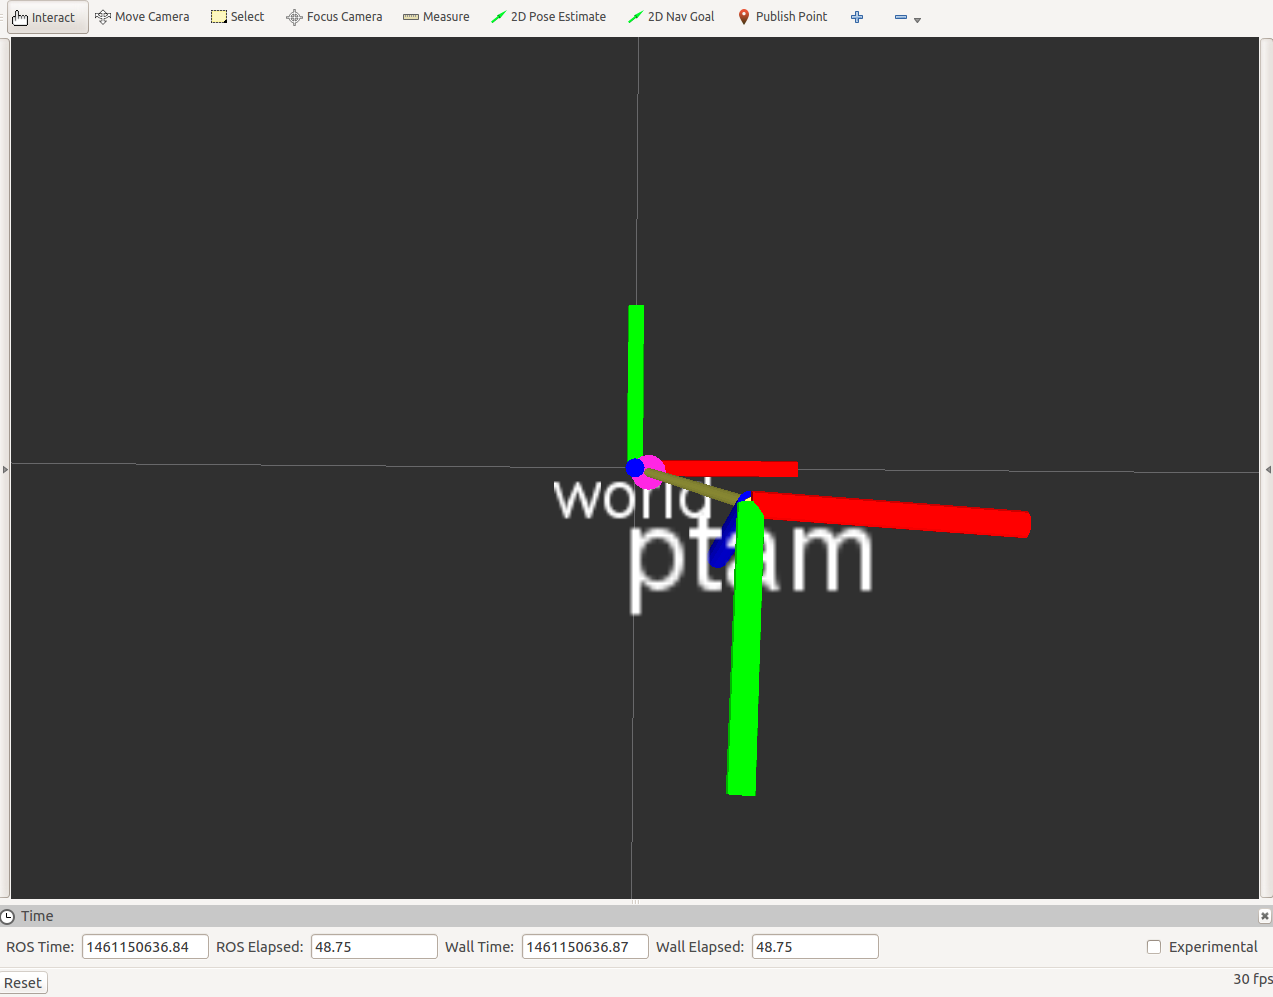
\includegraphics[width=.8\hsize]{rvizframe_}\label{fig:rviz_frame}}\\
   \subfigure[$Point\_W\_frame$]{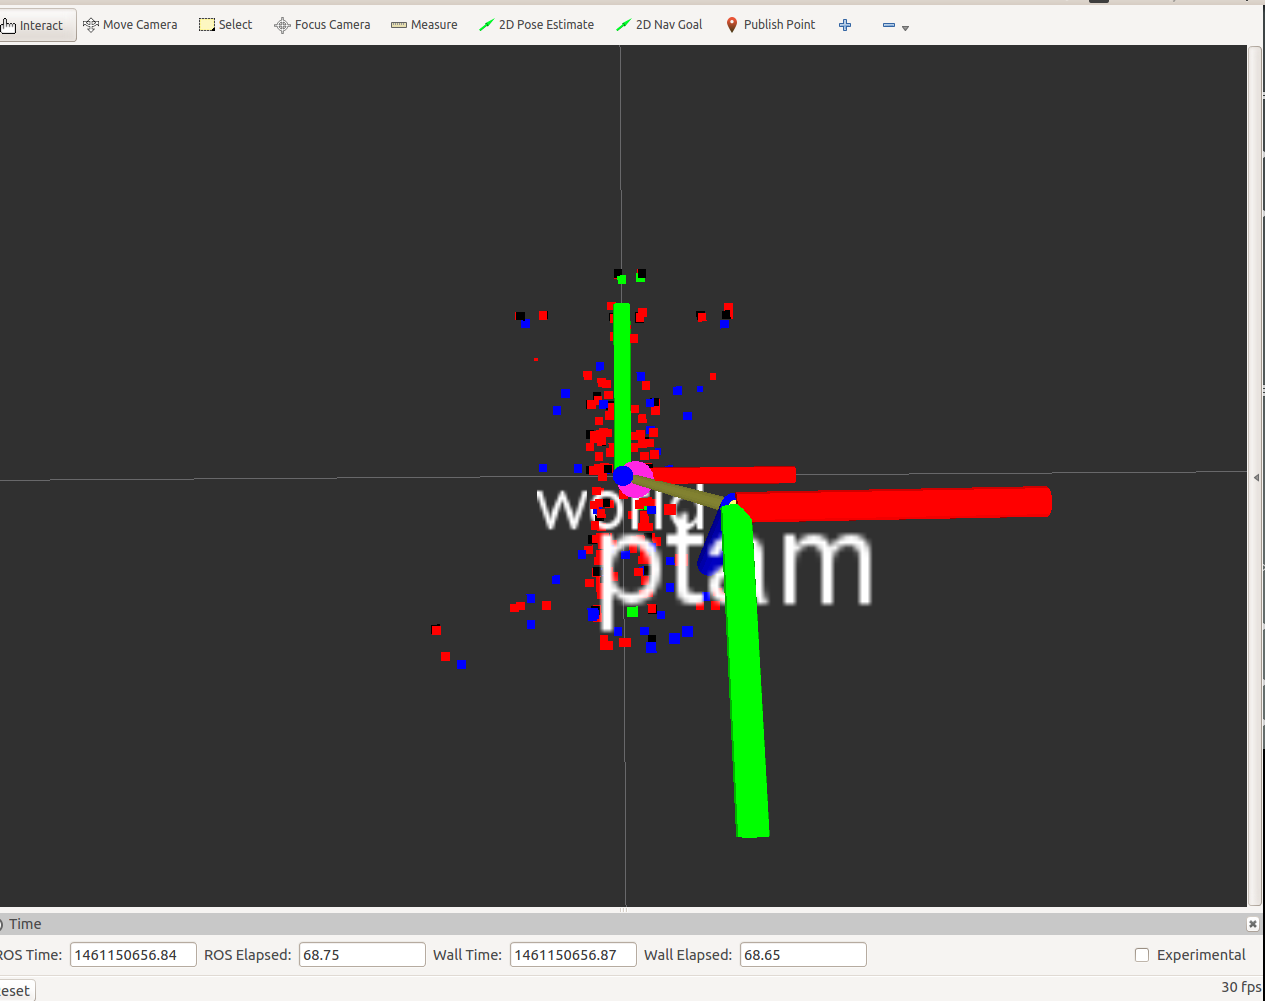
\includegraphics[width=.8\hsize]{rvizframepoint}\label{fig:rviz_Fpoint}}
\end{figure*}  
\begin{figure*}
 \centering
      \subfigure[$Point\_W\_frame$]{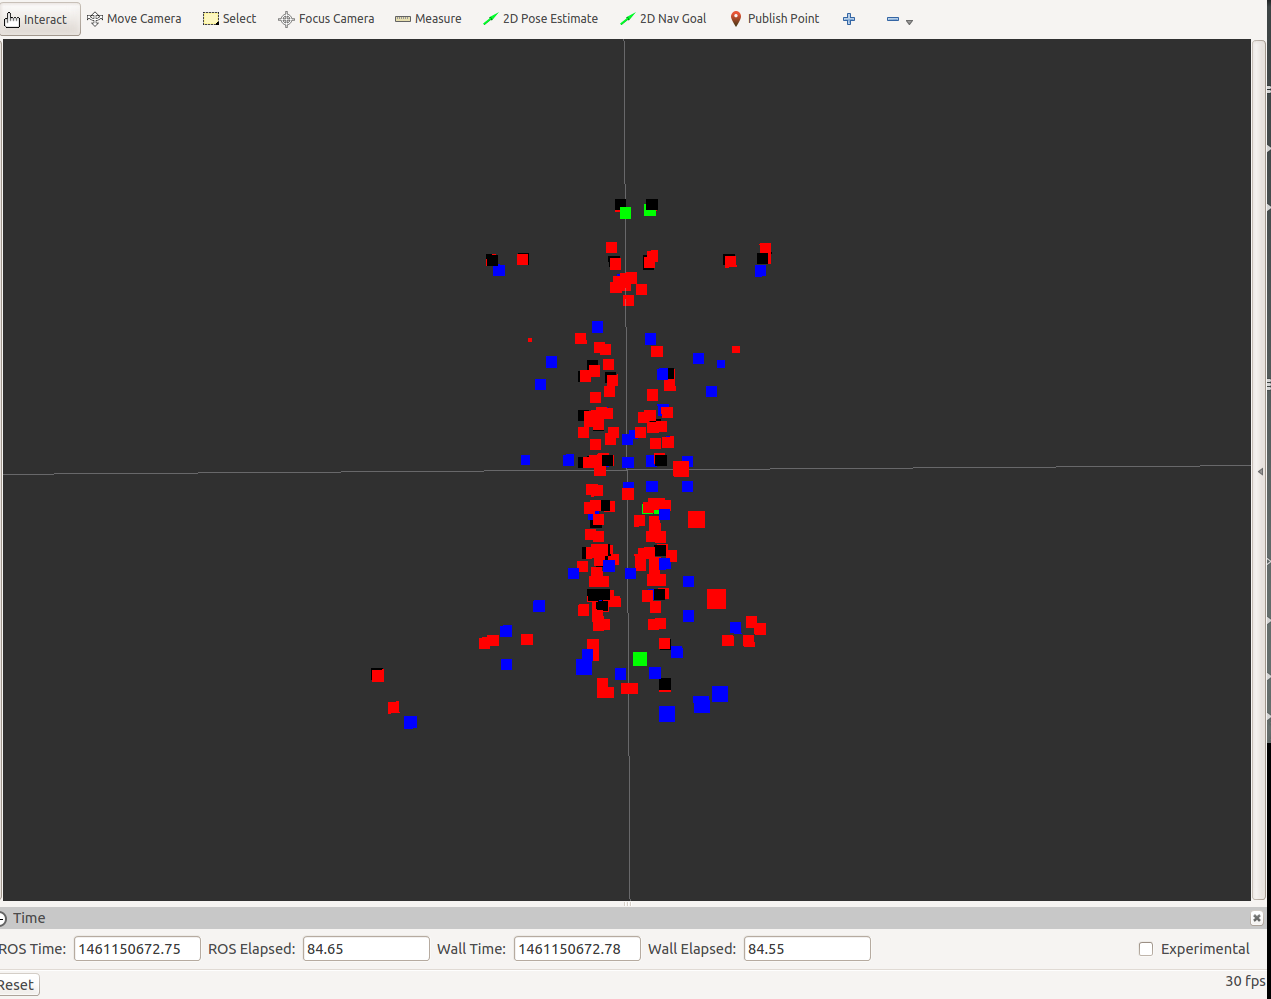
\includegraphics[width=.8\hsize]{rvizpoint}\label{fig:rviz_Fpoint}}
   \caption{Posizione delle features rispetto al word frame }
    \label{fig:rviz_point} 
\end{figure*}  
% \begin{figure}[H]
%    % \centering
%    \ContinuedFloat
%     \subfigure[$Point\_W\_frame$]{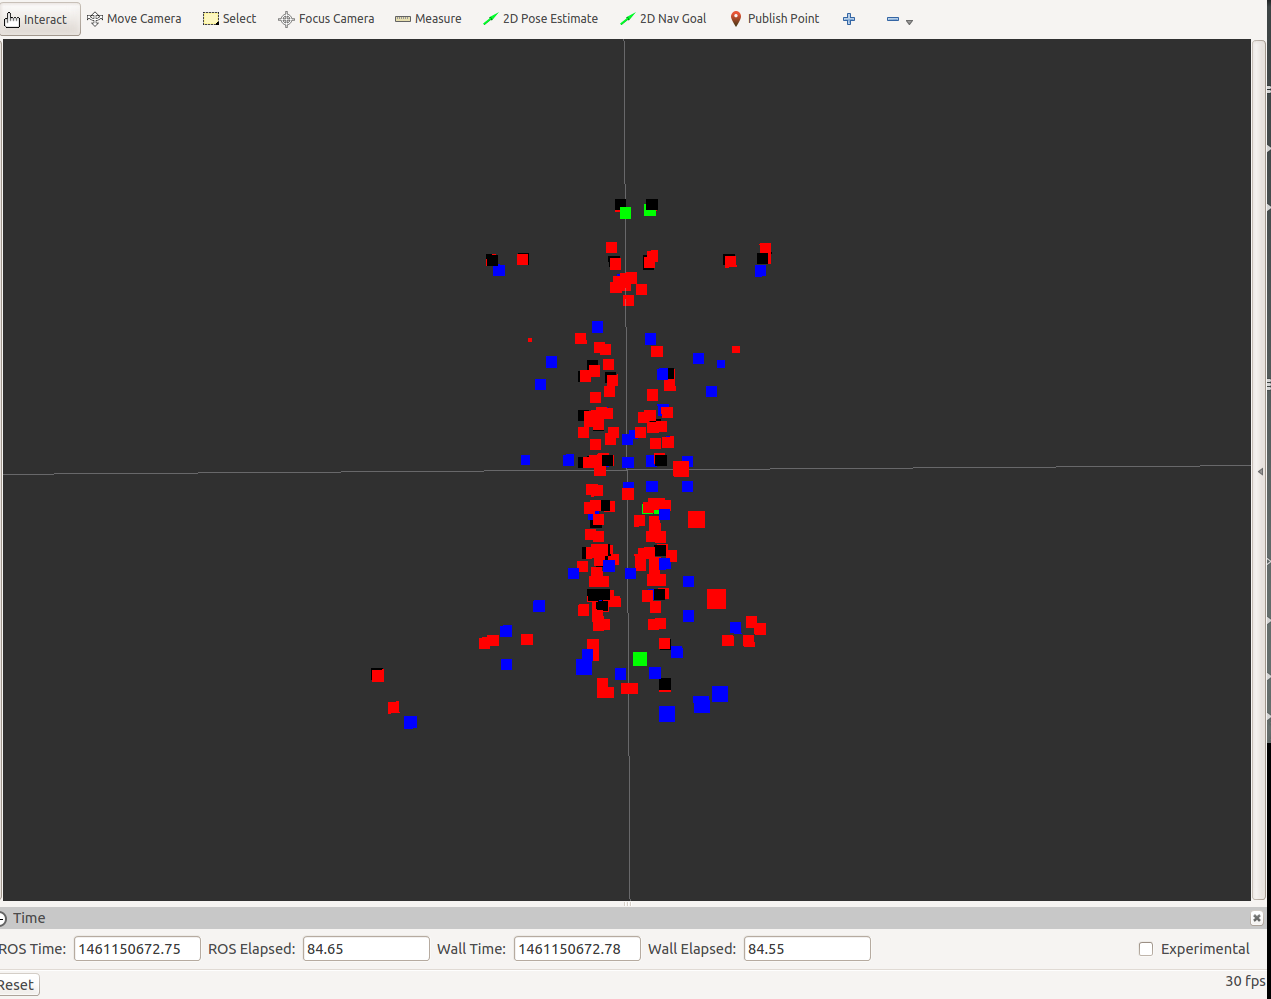
\includegraphics[width=.8\hsize]{rvizpoint}\label{fig:rviz_Fpoint}}
%    \caption{Posizione delle features rispetto al word frame }
%    \label{fig:rviz_point} 
% \end{figure}






\subsubsection{Stima del fattore di scala}
Come detto nel capitolo ~\ref{chapter1} questo algoritmo è soggetto ad un errore di scala. Se non correggessimo questo errore ci troveremmo in una posizione diversa rispetto alla posizione vera. Per questa ragione per correggere la scala si sono scritti due differenti metodi. 
Il primo metodo consente in un iterazione di stimare il valore della scala. Per questo metodo si utilizza il rapporto tra il reale spostamento del robot tra due sistemi di riferimento, e lo scostamento dato da Ptam.
\begin{equation}
s = \frac{Pr_{t-1} - Pr_{t}}{Pp_{t-1} - Pp_{t}}
\label{stima della scala primo metodo}
\end{equation}
Dove $Pr_{t-1} - Pr_{t}$ è lo spostamento reale del end-effector, mentre $Pp_{t-1} - Pp_{t}$ è lo spostamento secondo Ptam. Come vedremo nel capito ~\ref{chapter5} questo metodo è soggetto ad un errore di stima. Per ovviare a questo errore, si utilizzano dei metodi che permettono la convergenza della stima della scala al suo valore reale. Nel suo articolo Jacob Engel  ~\cite{scale} fornisce una stima dela fattore di scala utilizzando lo stimatore a massima verosimiglianza. Essenzialmente tale principio stabilisce di scegliere per un campione \underline{x} dato, quel valore di $\theta$ per cui massima era la probabilita' di estrarre proprio quel \underline{x}. Poiche' il logaritmo e' una funzione monotona, al posto del massimo di $L(\underline{x}, \theta)$ si preferisce cercare il massimo di $log L(\underline{x}, \theta)$. Dato una coppia di punti $(x_i, y_i)$, dove $x_i$ è la posizione affetta dal fattore di scala e $y_i$ è il valore reale, questi sono in relazione $x_i \approx \lambda y_i $. Se si ipotizza che il rumore di misura sia di tipo Gaussiano questi campioni possono essere scritti:
\begin{equation}
\begin{cases}
x_i \sim \Gamma(\lambda \mu_i, \sigma_x^2 I_{d*d})	\\
y_i \sim \Gamma(\mu_i, \sigma_y^2 I_{d*d})
\end{cases}
\label{rumore di misura}
\end{equation}
Dove $\mu_1 .... \mu_i$  $\epsilon$ $\Re^{d}$ rappresentano le vere ma ignote distanze, $\sigma_x^2$ e $\sigma_y^2$ rappresentano le varianze degli errori di misura.
Assumendo che le varianze siano note è possiile trovare una soluzione in forma chiusa dello stimatore minimizzando la funzione: 
\begin{equation}
L(\mu_1..\mu_n,\lambda)  \propto \frac{1}{2} \sum\limits_{i=1}^n (\frac{|| x_i - \lambda \mu_i ||^2}{\sigma_x^2}+ \frac{|| y_i - \mu_i|| ^2}{\sigma_y^2})
\label{funzione da minimizzare}
\end{equation}
Minimizzando per $\lambda$ è possibile trovare una soluzione unica
\begin{equation}
\lambda^* = \frac{s_{xx} - s_{yy} + sign(s_{xy}*\sqrt{(s_{xx} - s_{yy})^2 + 4*s_{xy}^2})}{2*\sigma_x^-1 * \sigma_y * s_{xy}}
\label{stima della scala per lo stimatore ML}
\end{equation}
Dove:
\begin{equation}
% \begin{cases}
s_{xx} = \sigma_y^2*\sum\limits_{i=1}^n x_i^t x_i	\qquad
s_{yy} = \sigma_x^2*\sum\limits_{i=1}^n y_i^t y_i	\qquad
s_{xy} = \sigma_y^2*\sigma_x^2 *\sum\limits_{i=1}^n x_i^t y_i^2
% \end{cases}
\label{}
\end{equation}
Questo metodo assicura la convergenza per un numero finito di passi. Nel capitolo ~\ref{chapter5} analizzeremo durante un esperimento i due metodi in esame.


\subsection{Posizione 3D del pulsante}
Per quanto detto finora PTAM tramite l'inizializzazione della mappa crea una collezione di punti 3D riferiti al frame mondo. La posizione delle features di interesse può essere acquisita da un utente esterno tramite la lettura del topic di riferimento. Questi punti sono inviati tramite un messaggio ROS in forma di point cloud\footnote{ Point cloud o nuvola di punti è un insieme di punti caratterizzati dalla loro posizione in un sistema di coordinate e da eventuali valori di intensità (colore, profondità, ecc.) ad essi associati. Esse servono solitamente come rappresentazione di strutture tridimensionali come oggetti o superfici } e, come si puo vedere da figura ~\ref{fig:point_cloud} rappresentano il 3D delle features trovate nella immagine.  
\begin{figure}[H]
   \centering
   \subfigure[$Features\_2d$]{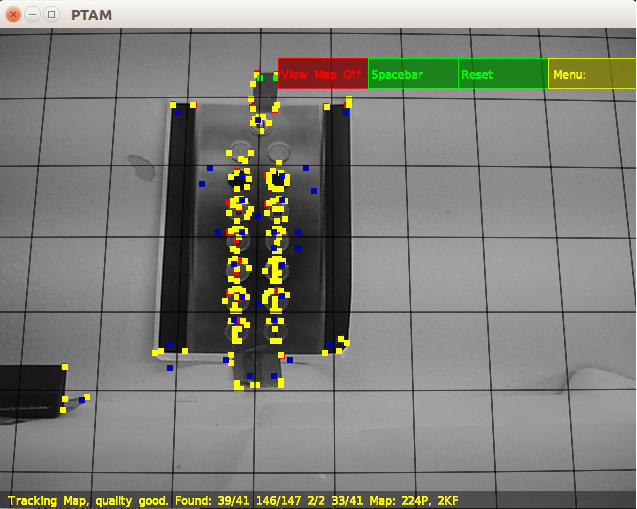
\includegraphics[width=.8\hsize]{ptamgrid}\label{fig:feature_2d}} 
   \subfigure[$Point\_cloud$]{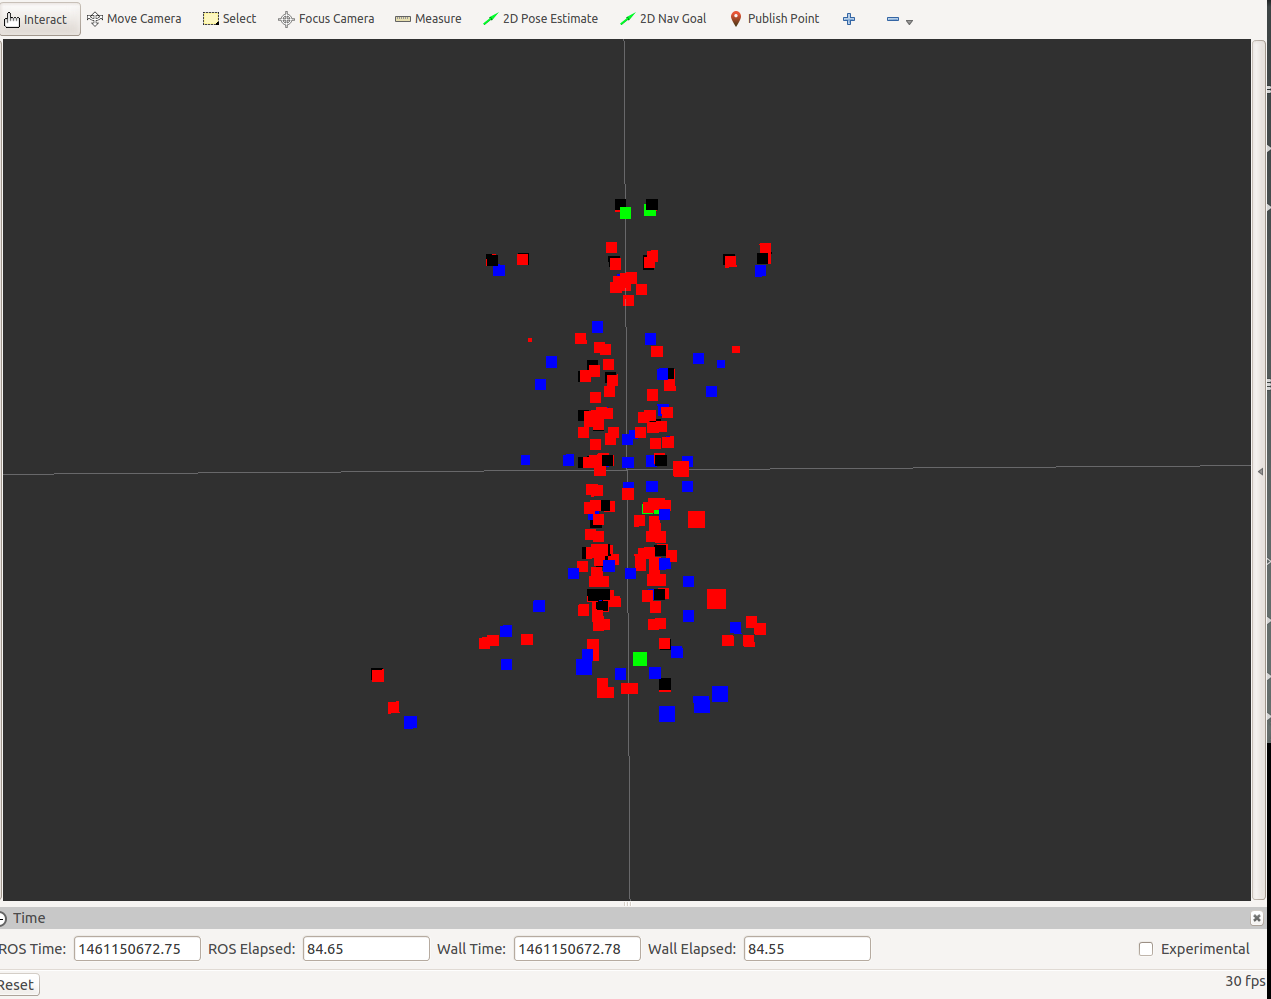
\includegraphics[width=.8\hsize]{rvizpoint}\label{fig:point_cloud}}
   \caption{Point cloud della mappa 3D}
   \label{fig:point_cloud} 
\end{figure}

Dalle informazioni della point cloud è possibile trovare le informazioni 2D riproiettando i punti nel piano immagine. Una volta che i punti vengono riproiettati si scelgono quelli più vicini al pulsante desiderato. Questa discriminazione viene fatta semplicemente calcolando tutte le distanze euclide dal pulsante. I punti scelti saranno quelli la cui distanza è minore di una soglia scelta, ci assicuriamo in questo modo di eliminare eventuali outlier presenti nel set di dati utilizzato. Grazie a questi punti è possibile trovare la posizione 3D del pulsante. Per ottenere questa infomazione si è deciso di fittare, tramite i minimi quadrati, un piano passante per questi punti. Utilizzando i parametri del piano assieme all'equazione ~\ref{eq:punto_immagine} è possibile trovare le coordinate 3D:
\begin{equation}
\begin{cases}
	a*X_c + b*Y_c + c*Z_c+ d = 0    \\
  	x_i = f_x * \frac{X_c}{Z_c}	+ c_x\\	
	y_i = f_y* \frac{Y_c}{Z_c} + c_y
 \end{cases}
 \label{sistema di equazione}
\end{equation}
Si hanno tre equazioni in tre incognite. 
\begin{equation}
\begin{cases}
	a*\frac{x_i - c_x}{f_x}*Z_c + b* \frac{y_i - c_y}{f_y}*Z_c + c*Z_c -d = 0   \\
  	X_c = \frac{x_i - c_x}{f_x} *Z_c\\	
	Y_c = \frac{y_i - c_y}{f_y} *Z_c
 \end{cases}
 \label{sistema di equazione}
\end{equation}
Da cui risolvendo per $Z_c$ si ottiene.
\begin{equation}
Z_c = \frac{d}{a*\frac{x_i - c_x}{f_x} + b* \frac{y_i - c_y}{f_y} +c }
\label{Profondita'}
\end{equation}
La posizione delle features che fornisce PTAM è rispetto al frame mondo, per i metodi implementati bisogna trasformarle nel sistema di riferimento camera tramite una trasformazione omogenea ~\ref{eq:wtocam}. Dove $T_c ^w$ rappresenta le cordinate del frame camera rispetto il frame mondo. 
\begin{equation}
P_c = T_c^w*P_w
\label{eq:wtocam}
\end{equation}